\chapter{Installing and Starting}
\label{ch:installing}

\section{The files}
\index{files!required}

\ccprod{} is seventeen files, and \textbf{all seventeen must be in the same
directory of the same device}.

\begin{cctable}{File}{What it is}{1.5in}{3.32in}
\fname{CMDRCALC.PRG} & The program. This is the one you load. \\
\fname{OVL1.BIN} \dots\ \fname{OVL16.BIN} & The rest of the program. \ccprod{}
is larger than the machine's memory, so it keeps most of itself on the card and
reads in whichever part it needs. \\
\end{cctable}

Together they come to about 135K. The names must be spelled exactly as they are
above, in capitals: the program builds them itself when it goes looking, and it
will not find a file named any other way.

\begin{cccaution}
Nothing is checked at startup. \ccprod{} starts perfectly happily with files
missing and then fails, silently, at the first command that needs one of them: a
menu that will not open, a file command that returns immediately having done
nothing, a formula that will not go into a cell. If the program is behaving as
though the keyboard is disconnected, count the files --- there should be
seventeen.
\end{cccaution}

\section{Installing on an SD card}
\index{SD card}

Copy the seventeen files into a directory of a CMDR-DOS-formatted card, put the
card in the machine, and:

\begin{ccprocedure}
\item Type \lit{LOAD"CMDRCALC.PRG",8} and press \key{Return}.
\item Type \lit{RUN} and press \key{Return}.
\end{ccprocedure}

\ccprod{} looks for the rest of itself on whichever device it was loaded from,
falling back to unit 8 if that cannot be determined --- which is almost always
the right answer anyway.

Your workbooks can live in the same directory. They do not have to; but the
file dialogue lists only the current directory and has no way to change it, so
in practice they will.

\section{Running under the emulator}
\index{emulator}\index{x16emu}

The \fname{x16emu} emulator serves a host directory to the program as though it
were unit 8, which is the most convenient way to work.

\begin{Verbatim}[fontsize=\small,xleftmargin=12pt]
x16emu -rom rom.bin -fsroot . -prg CMDRCALC.PRG -run
\end{Verbatim}

\lit{-fsroot} names the directory holding the seventeen files and your workbooks.
A \fname{rom.bin} is required: all of \ccprod's arithmetic is done by the
floating-point library in bank 4 of the Commander X16 ROM, and without a ROM
there is nothing to call.

Two flags change what you are testing.

\begin{cctable}{Flag}{Effect}{1.35in}{3.47in}
\lit{-ram 512} & The memory a real machine ships with. This is what to use if
you want to know whether a workbook will fit on stock hardware. \\
\lit{-ram 2048} & The emulator's maximum, and the machine's. The difference
between the two is the difference between a workbook of a few thousand cells
and one of a few hundred thousand. \\
\lit{-mhz 8} & The speed of a real Commander X16. Anything faster is a
convenience for development and will make imports look quicker than they are. \\
\end{cctable}

\begin{ccnote}
The \lit{-echo} flag will not show you \ccprod's display. The program draws
directly into video memory rather than going through the KERNAL's character
output, so there is nothing for \lit{-echo} to intercept. To capture the screen,
record with \lit{-gif} and take a frame from the recording.
\end{ccnote}

\section{Starting}

\ccprod{} starts with one empty worksheet named \msg{Sheet1}, the cursor on
\cellref{A1}, no file name, and the status line reading \msg{READY} with the
amount of free banked memory beside it.

\begin{ccfigure}
\ccscreenscale{1.4}
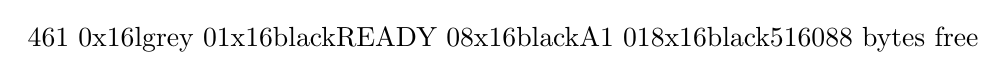
\begin{tikzpicture}
\node[inner sep=0pt,anchor=north west] (st) at (0,0) {%
\ccscreenbegin{46}{1}
  \ccfillrow{0}{x16lgrey}
  \cctext{0}{1}{x16black}{READY}
  \cctext{0}{8}{x16black}{A1}
  \cctext{0}{18}{x16black}{516088~bytes~free}
\ccscreenend
};
\end{tikzpicture}
\caption{The status line at startup on a 512K machine}
\end{ccfigure}

The figure that appears there is the whole of banked RAM, measured once. On a
2M machine it reads something over two million. It is a statement of how large
a workbook this machine can hold, and it does not change as you fill the
workbook up.

\section{Quitting}
\index{quitting}

Press \key{F9}, or choose \menupath{File > Quit}.

If the workbook has been modified --- if the status line says \msg{MODIF} ---
\ccprod{} asks first:

\begin{ccfigure}
\ccscreenscale{1.15}
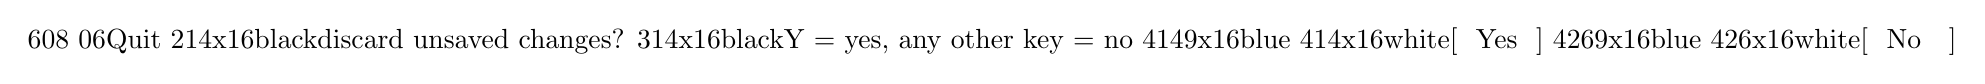
\begin{tikzpicture}
\node[inner sep=0pt,anchor=north west] (dq) at (0,0) {%
\ccscreenbegin{60}{8}
  \ccdlgbox{0}{6}{Quit}
  \cctext{2}{14}{x16black}{discard~unsaved~changes?}
  \cctext{3}{14}{x16black}{Y~=~yes,~any~other~key~=~no}
  \ccfill{4}{14}{9}{x16blue}
  \cctext{4}{14}{x16white}{[~~Yes~~]}
  \ccfill{4}{26}{9}{x16blue}
  \cctext{4}{26}{x16white}{[~~No~~~]}
\ccscreenend
};
\end{tikzpicture}
\caption{The confirmation shown when quitting with unsaved changes}
\label{fig:quitconfirm}
\end{ccfigure}

\key{Y} quits and throws the work away. \emph{Any} other key cancels --- there
is no separate \key{N}; anything that is not \key{Y} means no. You can also
click the buttons.

On exit the screen is cleared to white on blue and you are back in BASIC.

\section{If something is wrong}

\begin{cctable}{Symptom}{Cause}{1.85in}{2.97in}
Menus will not open; file commands do nothing & One of the program's files is
missing or mis-named. Check that all sixteen \fname{OVL}\emph{n}\fname{.BIN}
files are present beside \fname{CMDRCALC.PRG}, spelled in capitals. \\
\msg{no matching files on the card} when opening a workbook you know is there &
The dialogue lists only the current directory, only files ending \fname{.X16S},
and only the first sixty-four entries. See Chapter~\ref{ch:files}. \\
The status line says \msg{STACK!} & An internal limit has been
exceeded. Save your work under a new name and restart. See Chapter~\ref{ch:messages}. \\
Arithmetic gives nonsense, or the machine drops to BASIC & There is no ROM, or
the wrong one. The floating-point library lives in ROM bank 4. \\
Nothing is legible & The machine is in a text mode \ccprod{} did not expect.
It wants 80 by 60. \\
\end{cctable}
